In this section, we formalize \textit{query split}. We first define the concept of select-projection-join query and formally describe \textit{query split} for such queries (in Section \ref{S31}). Then, we design an implementation for reconstruction algorithm, which is one of the components of \textit{query split}, and prove its correctness (in Section \ref{S32}).
\subsection{Framework Overview} \label{S31}
    In this section, we give an overview of \textit{query split} framework. For simplicity, we temporarily restrict our attention to select-projection-join (SPJ) queries in the following three sections, which only involve select, projection, and join operators. These three operators are chosen because they can be connected together to compose most of the basic SQL SELECT queries, covering all the queries in the Join Order Benchmark \cite{JOB}. \textit{Query split} can be extended to handle more general queries, which is discussed in Section \ref{S6}.\par
    First, let us define a normal form of SPJ queries. Then by relational algebra manipulation, every SPJ queries can be transformed into the following normal form, in which we denote by \textbf{\textit{R}} a set of relations, \textbf{\textit{S}} a set of select predicates over \textbf{\textit{R}} and \textbf{\textit{P}} a set of projection attributes, via equivalence rules (details can be found in Appendix A).
    $$q(\textbf{\textit{R}},\textbf{\textit{S}},\textbf{\textit{P}})=\Pi_{\textbf{{\textit{P}}}}(\sigma_{\textbf{\textit{S}}}(r_1 \times r_2 \times... \times r_m)),r_i \in \textbf{\textit{R}}$$
    Now, we can formally describe \textit{query split}. The framework consists of five components: query splitting algorithm, run-time statistics collector, query optimizer, query executor, and the reconstruction algorithm. The relationship between five components are shown in Figure \ref{F4}. Query splitting algorithm takes the global query as input and splits it into sub-queries, and then we obtain the result via the following steps:
    \begin{enumerate}[leftmargin = 15pt]
        \item In each iteration, the reconstruction algorithm picks a sub-query and sends it to the query optimizer.
        \item The query optimizer makes an execution plan and delivers it to the query executor.
        \item The query executor executes the plan, materialize the results and sends them to statistic collector.
        \item The run-time statistic collector obtains new statistics, which can help the optimizer make better plans for the remaining sub-queries in the following iterations.
        \item After all subqueries have been executed, the reconstruction algorithm reconstructs the final query result relation from sub-query results.
    \end{enumerate}
    \begin{figure}[htb]
        \centering
        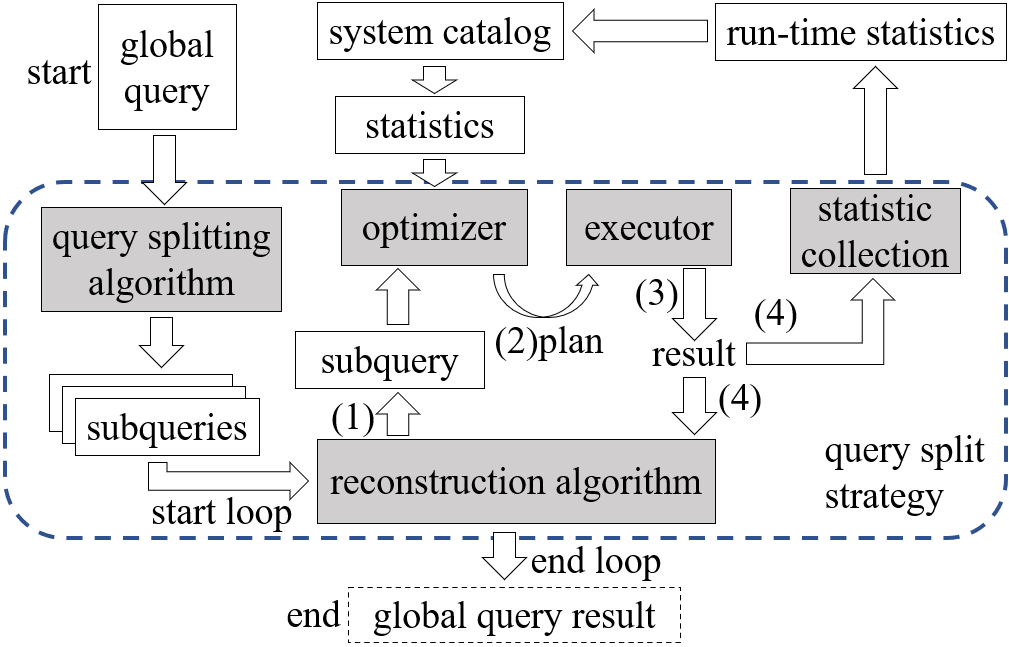
\includegraphics[width=\linewidth]{./pic/Figure4.png}
        \caption{The framework of \textit{query split}}
        \label{F4}
        \Description{}
    \end{figure}\par
    Note that statistics collector, query optimizer, and query executor are existing components in RDBMS. In the following, we define query splitting algorithm and reconstruction algorithm, the two new concepts that we propose in this paper.\par
    We first formalize the concept of sub-query and query splitting algorithm, in which we stipulate that sub-queries do not contain projection operations. The definition of query splitting algorithm here is abstract, and we will discuss possible concrete implementations in Section 4.1.
    \begin{Definition} \label{D1}
        Given two $SPJ$ queries q(\textbf{\textit{R}}, \textbf{\textit{S}}, \textbf{\textit{P}}) and q$'($\textbf{\textit{R}}$',$\textbf{\textit{S}}$')$. If \textbf{\textit{R}}$'\subseteq$\textbf{\textit{R}} and \textbf{\textit{S}}$'\subseteq$\textbf{\textit{S}}, then q$'$ is said to be a sub-query of query q. Query splitting algorithm is an algorithm which takes a SP$J$ query q as input and returns a set of sub-queries of q.
    \end{Definition}\par
    Next, we define the concept of reconstruction algorithm.\par
    \begin{Definition} \label{D2}
        Reconstruction algorithm is an algorithm that takes a set of sub-queries \textbf{\textit{Q}} and a set of projection attributes \textbf{\textit{P}} as input and returns a reconstructed relation. A reconstruction algorithm A is correct with respect to a query splitting algorithm B if, for every SP$J$ query q(\textbf{\textit{R}}, \textbf{\textit{S}}, \textbf{\textit{P}}), the reconstructed relation is always equal to the result of the original query, if we feed the output of B on q together with \textbf{\textit{P}} as input of A.
    \end{Definition}\par
    Clearly, not every query splitting algorithm has a corresponding reconstruction algorithm. A crucial question here is under which conditions a correct reconstruction algorithm exists. To answer this question, we define the concept of subquery cover.
    \begin{Definition} \label{D3}
        Given a SP$J$ query q(\textbf{\textit{R}}, \textbf{\textit{S}}, \textbf{\textit{P}}), let \textbf{\textit{Q}}=$\{q_1(\textbf{\textit{R}}_1,\textbf{\textit{S}}_1)$, ..., $q_n(\textbf{\textit{R}}_n,\textbf{\textit{S}}_n)\}$ be a set of subqueries of q. We denoted R(\textbf{\textit{Q}})=$\cup_{i=1}^n \textbf{\textit{R}}_i$ and S(\textbf{\textit{Q}})=$\cup_{i=1}^n \textbf{\textit{S}}_i$. \textbf{\textit{Q}} is said to cover $q$ (\textbf{\textit{Q}}$\rightharpoonup_c$q) if,\par
        (1) R(\textbf{\textit{Q}})=\textbf{\textit{R}}\par
        (2) S(\textbf{\textit{Q}}) logically implies \textbf{\textit{S}}. \footnote[1]{``A logically implies B" means that each predicate from B can be inferred by A.}
    \end{Definition}\par
    Intuitively, the reconstruction can succeed only if there is no information loss between the set of sub-queries and the original query, and the sub-query cover concept formalizes this intuition. To ensure a correct reconstruction algorithm exist, the set of sub-queries \textbf{\textit{Q}} returned by a query splitting algorithm with query q needs to satisfy \textbf{\textit{Q}}$\rightharpoonup_c$q. And we give a simple reconstruction algorithm that guarantees correctness under such conditions in the following section.

\subsection{Replacement Reconstruction} \label{S32}
    In this section, we propose a concrete reconstruction algorithm called \textit{replacement reconstruction}, which is correct with respect to every query splitting algorithm that are guaranteed to cover the original query. The correctness of this algorithm will be proved later.
    \begin{figure}[htb]
        \centering
        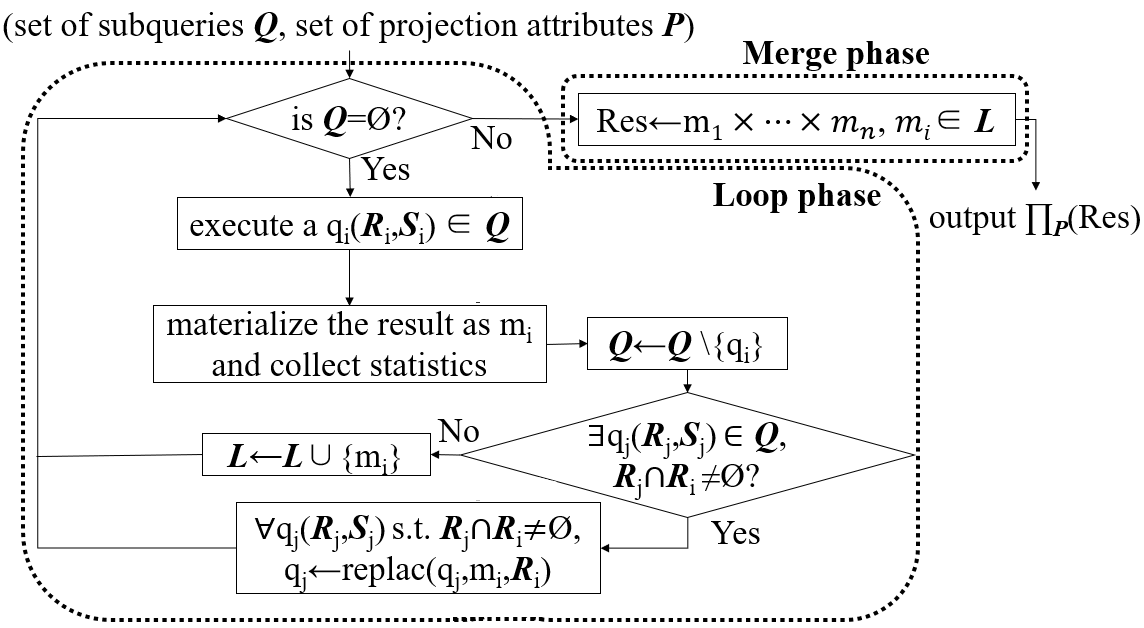
\includegraphics[width=\linewidth]{./pic/Figure5.png}
        \caption{Replacement reconstruction}
        \label{F5}
        \Description{}
    \end{figure}\par
    Figure \ref{F5} shows a flow chart that explains how \textit{replacement reconstruction} algorithm works. The algorithm takes the set of sub-queries \textbf{\textit{Q}} and the set of projection attributes \textbf{\textit{P}} as inputs, and use the following steps to reconstruct the query result.
    \begin{algorithm}[htb]
        \caption{Replacement Reconstruction}
        \begin{algorithmic}[1]
            \Require \textbf{\textit{Q}} a set of sub-queries, \textbf{\textit{P}} a set of projection attributes
            \Function{ReplacRecon}{\textbf{\textit{Q}}, \textbf{\textit{P}}}
                \State \textbf{\textit{L}} $\gets \emptyset$
                \While{\textbf{\textit{Q}} $\neq \emptyset$}
                    \State $\backslash$* use QSELECT() to choose a sub-query from \textbf{\textit{Q}} *$\backslash$
                    \State $q_i(\textbf{\textit{R}}_i,\textbf{\textit{S}}_i) \gets$ \Call{QSELECT}{\textbf{\textit{Q}}}
                    \State $\backslash$* EXEC() executes sub-query and materialize results *$\backslash$
                    \State $m_i \gets$ \Call{EXEC}{$q_i$}
                    \State $\backslash$* STAT() collects the run-time statistics*$\backslash$
                    \State $system\_catalog \gets$ \Call{STAT}{$m_i$}
                    \State \textbf{\textit{Q}} $\gets$ \textbf{\textit{Q}} $\setminus \{q_i\}$
                    \State $flag \gets 0$
                    \For{$q_j(\textbf{\textit{R}}_j,\textbf{\textit{S}}_j) \in$ \textbf{\textit{Q}}}
                        \If{$\textbf{\textit{R}}_j \cap \textbf{\textit{R}}_i \neq \emptyset$}
                            \State $\backslash$* replace subset $\textbf{\textit{R}}_j \cap \textbf{\textit{R}}_i$ in $\textbf{\textit{R}}_j$ with $m_i$ *$\backslash$
                            \State $q_j \gets$ replac($q_j$, $m_i$, $\textbf{\textit{R}}_i$)
                            \State $flag \gets 1$
                        \EndIf
                    \EndFor
                    \If{$flag=0$}
                        \State \textbf{\textit{L}} $\gets$ \textbf{\textit{L}} $\cup \{m_i\}$
                    \EndIf
                \EndWhile
                \State $Res \gets m_1 \times m_2 \times ... \times m_n, m_i \in$ \textbf{\textit{L}}
                \State \Return{$\Pi_{\textbf{\textit{P}}}(Res)$}
            \EndFunction
        \end{algorithmic}
    \end{algorithm}
    \begin{itemize}[leftmargin = 15pt]
        \item \textbf{Initial}: initialize the set of sub-query results \textbf{\textit{L}} as empty set.
        \item \textbf{Loop(execute)}: execute a sub-query $q_i(\textbf{\textit{R}}_i,\textbf{\textit{S}}_i)$ from \textbf{\textit{Q}} and materialize the result as $m_i$, then collect run-time statistics. 
        \item \textbf{Loop(modify)}: remove $q_i(\textbf{\textit{R}}_i,\textbf{\textit{S}}_i)$ from \textbf{\textit{Q}}, then pick out all sub-queries $q_j(\textbf{\textit{R}}_j,\textbf{\textit{S}}_j)$ whose set of relations $\textbf{\textit{R}}_j$ intersects with $\textbf{\textit{R}}_i$, modify these sub-queries via a specific protocol that will be described later $q_j \gets$ replac$(q_j, m_i, \textbf{\textit{R}}_i)$. If there is no such $q_j$, add $m_i$ to \textbf{\textit{L}}. After this, check whether \textbf{\textit{Q}} is empty and repeat the loop if not.
        \item \textbf{Merge}: when \textbf{\textit{Q}} is empty, compute the Cartesian product of all relations in \textbf{\textit{L}} and project on the result by \textbf{\textit{P}}, and the end result is the reconstructed relation.
    \end{itemize}\par
    It remains to describe how replac$(q_j, m_i, \textbf{\textit{R}}_i)$ works. It actually modifies the sub-query $q_j(\textbf{\textit{R}}_j,\textbf{\textit{S}}_j)$ from two aspects.
    \begin{itemize}[leftmargin = 15pt]
        \item First, replace all relations in $\textbf{\textit{R}}_i \cap \textbf{\textit{R}}_j$ by $m_i$. In other words, set the set of relations of $q_j$ as $\textbf{\textit{R}}_j \gets \textbf{\textit{R}}_j \setminus \textbf{\textit{R}}_i \cup \{m_i\}$.
        \item After replacing old relations from $\textbf{\textit{R}}_j$ with $m_i$, some predicates in $\textbf{\textit{S}}_j$ would be referencing removed relations. Update those predicates by using the corresponding attributes in $m_i$ instead.
    \end{itemize}\par
    Now we can prove the correctness of replacement reconstruction algorithm.
    \begin{Theorem}[1] \label{Th1}
        Let q(\textbf{\textit{R}}, \textbf{\textit{S}}, \textbf{\textit{P}}) be an SP$J$ query, \textbf{\textit{Q}} be a set of sub-queries of q. If \textbf{\textit{Q}}$\rightharpoonup_c$q, then the output of the replacement reconstruction algorithm is equal to the result of q.
    \end{Theorem}\par
    This implies that the replacement reconstruction algorithm is a correct reconstruction algorithm for any query splitting algorithm that guarantees its output to cover the original query. The proof of this theorem can be found in Appendix B.\vspace{6pt}\\
    \textit{Remark}: In Definition \ref{D1}, we assume that there is no projection operation in sub-queries for simplicity. In practice, we can push down the projection operation to each sub-query to effectively reduce the size of the temporary relation and minimize execution time. In principle, any attribute which doesn't appear in other sub-queries can be safely projected away.